\documentclass[tikz,border=6pt]{standalone}
\usepackage{tikz}
\usetikzlibrary{arrows.meta,backgrounds,calc,fit,positioning,shapes.geometric,shapes.misc}

\definecolor{macroblue}{HTML}{4C78A8}
\definecolor{midgreen}{HTML}{59A14F}
\definecolor{microorange}{HTML}{F28E2B}
\definecolor{softgray}{HTML}{F4F4F4}
\definecolor{chipgray}{HTML}{E4E6E8}
\definecolor{edgegray}{HTML}{B8BDC3}
\definecolor{textgray}{HTML}{4D4D4D}

\colorlet{hiddenflowcolor}{macroblue!92!black}
\colorlet{featureflowcolor}{microorange!95!black}
\colorlet{metaflowcolor}{black!55}

\tikzset{
  >={Latex[length=2.5mm,width=2.2mm]},
  every node/.style={inner sep=0pt,outer sep=0pt},
  figure label/.style={font=\scriptsize\sffamily\bfseries,text=textgray},
  section label/.style={font=\scriptsize\sffamily,text=textgray},
  band text/.style={font=\scriptsize\sffamily\bfseries,text=black!85,align=center},
  tokenbox/.style={rounded corners=2pt, draw=edgegray, fill=white, line width=0.6pt},
  sourcebox/.style={rounded corners=5pt, draw=edgegray, fill=white, line width=0.6pt},
  panelbox/.style={rounded corners=7pt, draw=black!12, fill=white, line width=0.7pt},
  neutralchip/.style={rounded corners=2pt, draw=edgegray!90, fill=chipgray, line width=0.45pt},
  cuepill/.style={rounded corners=3pt, draw=edgegray!90, fill=softgray, line width=0.5pt},
  legendtext/.style={font=\scriptsize\sffamily,text=textgray},
  stagehead/.style={rounded corners=4pt, line width=0.6pt},
  attnbox/.style={rounded corners=4pt, draw=edgegray!95, fill=softgray, line width=0.6pt},
  simplebox/.style={rounded corners=4pt, draw=edgegray!95, fill=white, line width=0.6pt},
  routerbox/.style={rounded corners=3pt, draw=edgegray!95, fill=softgray, line width=0.55pt},
  expertbox/.style={rounded corners=2pt, draw=edgegray!95, fill=white, line width=0.5pt},
  hiddenflow/.style={->, draw=hiddenflowcolor, line width=1.1pt},
  featureflow/.style={->, draw=featureflowcolor, line width=1.0pt, dash pattern=on 3.2pt off 1.8pt},
  metaflow/.style={->, draw=metaflowcolor, line width=0.55pt},
}

\newcommand{\fmoeTokenNode}[3]{%
  \begin{scope}[shift={({#1},{#2})}]
    \path[tokenbox] (-0.42,-0.34) rectangle (0.42,0.34);
    #3
  \end{scope}%
}

\newcommand{\fmoeBallIcon}{%
  \draw[line width=0.45pt, draw=textgray] (0,0) circle [radius=0.16];
  \draw[line width=0.35pt, draw=textgray] (-0.11,0) -- (0.11,0);
  \draw[line width=0.35pt, draw=textgray] (0,-0.11) -- (0,0.11);
  \draw[line width=0.3pt, draw=textgray] (-0.09,-0.09) -- (0.09,0.09);
  \draw[line width=0.3pt, draw=textgray] (-0.09,0.09) -- (0.09,-0.09);
}

\newcommand{\fmoeBootsIcon}{%
  \filldraw[draw=textgray, fill=black!10, line width=0.35pt]
    (-0.16,-0.03) -- (-0.02,-0.03) -- (0.02,-0.11) -- (-0.15,-0.11) -- cycle;
  \filldraw[draw=textgray, fill=black!10, line width=0.35pt]
    (0.01,0.04) -- (0.16,0.04) -- (0.19,-0.05) -- (0.02,-0.05) -- cycle;
}

\newcommand{\fmoeJerseyIcon}{%
  \filldraw[draw=textgray, fill=black!8, line width=0.35pt]
    (-0.13,0.12) -- (-0.04,0.12) -- (0,0.05) -- (0.04,0.12) -- (0.13,0.12) --
    (0.17,0.02) -- (0.09,-0.03) -- (0.08,-0.16) -- (-0.08,-0.16) -- (-0.09,-0.03) -- (-0.17,0.02) -- cycle;
}

\newcommand{\fmoeGuardIcon}{%
  \filldraw[draw=textgray, fill=black!9, line width=0.35pt]
    (0,0.16) -- (0.12,0.1) -- (0.09,-0.1) -- (0,-0.17) -- (-0.09,-0.1) -- (-0.12,0.1) -- cycle;
}

\newcommand{\fmoeSocksIcon}{%
  \filldraw[draw=textgray, fill=black!8, line width=0.35pt]
    (-0.13,0.14) rectangle (-0.04,-0.02);
  \filldraw[draw=textgray, fill=black!8, line width=0.35pt]
    (-0.04,-0.02) -- (0.03,-0.02) -- (0.03,-0.09) -- (-0.1,-0.09) -- cycle;
  \filldraw[draw=textgray, fill=black!8, line width=0.35pt]
    (0.04,0.14) rectangle (0.13,-0.02);
  \filldraw[draw=textgray, fill=black!8, line width=0.35pt]
    (0.04,-0.02) -- (0.11,-0.02) -- (0.11,-0.09) -- (-0.02,-0.09) -- cycle;
}

\newcommand{\fmoeOrderIcon}{%
  \draw[textgray, line width=0.45pt] (-0.16,0.09) -- (0.12,0.09);
  \draw[textgray, line width=0.45pt] (-0.16,0) -- (0.12,0);
  \draw[textgray, line width=0.45pt] (-0.16,-0.09) -- (0.12,-0.09);
  \fill[textgray] (-0.2,0.09) circle[radius=0.018];
  \fill[textgray] (-0.2,0) circle[radius=0.018];
  \fill[textgray] (-0.2,-0.09) circle[radius=0.018];
}

\newcommand{\fmoeClockIcon}{%
  \draw[textgray, line width=0.45pt] (0,0) circle[radius=0.15];
  \draw[textgray, line width=0.45pt] (0,0) -- (0,0.07);
  \draw[textgray, line width=0.45pt] (0,0) -- (0.06,-0.04);
}

\newcommand{\fmoeGridIcon}{%
  \foreach \x in {-0.12,0.02} {
    \foreach \y in {-0.1,0.04} {
      \path[draw=textgray, fill=black!6, line width=0.35pt] (\x,\y) rectangle +(0.1,0.1);
    }
  }
}

\newcommand{\fmoeBarsIcon}{%
  \filldraw[draw=textgray, fill=black!12, line width=0.35pt] (-0.16,-0.13) rectangle (-0.08,0.0);
  \filldraw[draw=textgray, fill=black!12, line width=0.35pt] (-0.03,-0.13) rectangle (0.05,0.08);
  \filldraw[draw=textgray, fill=black!12, line width=0.35pt] (0.10,-0.13) rectangle (0.18,0.14);
}

\newcommand{\fmoeSourceBox}[4]{%
  \begin{scope}[shift={({#1},{#2})}]
    \path[sourcebox] (-0.95,-0.36) rectangle (0.95,0.36);
    \begin{scope}[shift={(-0.52,0)}]
      #4
    \end{scope}
    \node[anchor=west, font=\scriptsize\sffamily\bfseries, text=textgray] at (-0.18,0) {#3};
  \end{scope}%
}

\newcommand{\fmoeChipGrid}[2]{%
  \begin{scope}[shift={({#1},{#2})}]
    \foreach \x/\y in {-0.26/0.12,0.26/0.12,-0.26/-0.14,0.26/-0.14} {
      \path[neutralchip] (\x-0.18,\y-0.06) rectangle +(0.36,0.12);
    }
  \end{scope}%
}

\newcommand{\fmoeStageCard}[5]{%
  \begin{scope}[shift={({#1},{#2})}]
    \path[simplebox] (-1.05,-0.72) rectangle (1.05,0.72);
    \path[draw=#3!80!black, fill=#3!16, rounded corners=4pt, line width=0.6pt] (-0.92,0.2) rectangle (0.92,0.58);
    \node[font=\scriptsize\sffamily\bfseries, text=black!88] at (0,0.39) {#4};
    \fmoeChipGrid{0}{-0.13}
    #5
  \end{scope}%
}

\newcommand{\fmoeLegendSample}[4]{%
  \draw[#2] (#1, #3) -- ++(0.9,0);
  \node[anchor=west, legendtext] at ($(#1,#3)+(1.05,0)$) {#4};
}

\newcommand{\fmoeCaption}[2]{%
  \par\noindent\parbox{#1}{\footnotesize\sffamily #2}%
}


\begin{document}
\sffamily
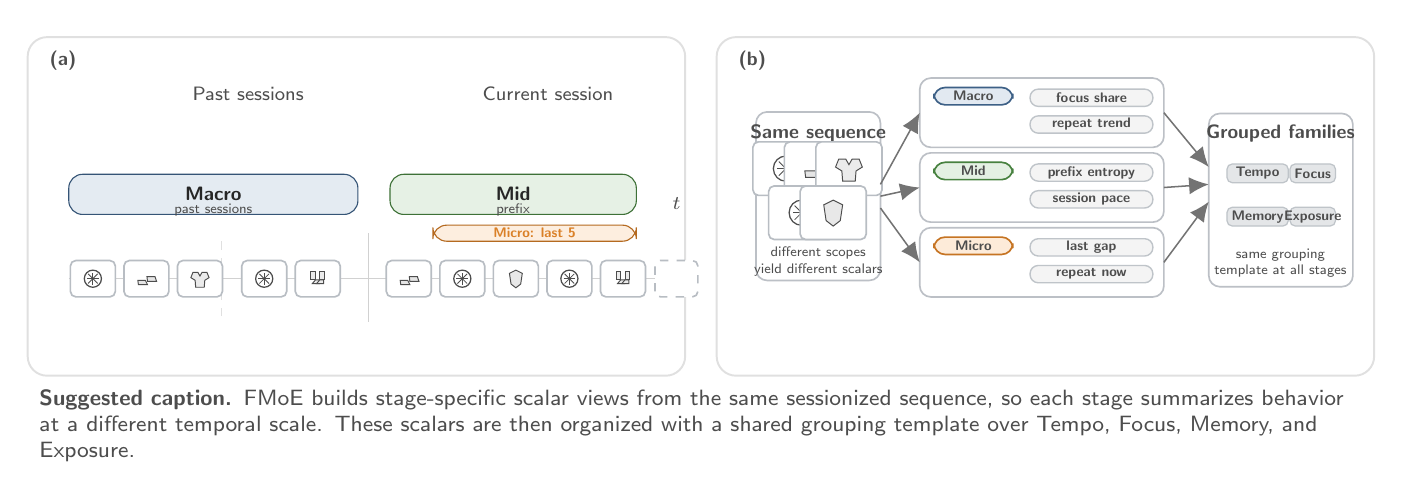
\begin{tikzpicture}[x=1cm,y=1cm]
  \path[use as bounding box] (0,-1.22) rectangle (17.15,4.42);
  \path[panelbox] (0,0) rectangle (8.35,4.3);
  \path[panelbox] (8.75,0) rectangle (17.1,4.3);
  \node[figure label, anchor=west] at (0.28,4.0) {(a)};
  \node[figure label, anchor=west] at (9.03,4.0) {(b)};

  \begin{scope}[shift={(0.42,0.45)}, x=0.68cm, y=0.68cm]
    \node[section label] at (3.5,4.6) {Past sessions};
    \node[section label] at (9.1,4.6) {Current session};
    \draw[black!18, line width=0.45pt] (0.15,1.15) -- (11.55,1.15);
    \draw[black!12, dashed, line width=0.4pt] (3.0,0.45) -- (3.0,1.95);
    \draw[black!18, line width=0.5pt] (5.75,0.35) -- (5.75,2.0);

    \filldraw[draw=macroblue!70!black, fill=macroblue!15, rounded corners=5pt] (0.15,2.35) rectangle (5.55,3.1);
    \node[band text] at (2.85,2.73) {Macro};
    \node[font=\tiny\sffamily, text=textgray] at (2.85,2.43) {past sessions};

    \filldraw[draw=midgreen!70!black, fill=midgreen!15, rounded corners=5pt] (6.15,2.35) rectangle (10.75,3.1);
    \node[band text] at (8.45,2.73) {Mid};
    \node[font=\tiny\sffamily, text=textgray] at (8.45,2.43) {prefix};

    \filldraw[draw=microorange!75!black, fill=microorange!15, rounded corners=5pt] (6.95,1.85) rectangle (10.75,2.15);
    \node[font=\tiny\sffamily\bfseries, text=microorange!90!black] at (8.85,2.0) {Micro: last 5};

    \fmoeTokenNode{0.6}{1.15}{\fmoeBallIcon}
    \fmoeTokenNode{1.6}{1.15}{\fmoeBootsIcon}
    \fmoeTokenNode{2.6}{1.15}{\fmoeJerseyIcon}
    \fmoeTokenNode{3.8}{1.15}{\fmoeBallIcon}
    \fmoeTokenNode{4.8}{1.15}{\fmoeSocksIcon}

    \fmoeTokenNode{6.5}{1.15}{\fmoeBootsIcon}
    \fmoeTokenNode{7.5}{1.15}{\fmoeBallIcon}
    \fmoeTokenNode{8.5}{1.15}{\fmoeGuardIcon}
    \fmoeTokenNode{9.5}{1.15}{\fmoeBallIcon}
    \fmoeTokenNode{10.5}{1.15}{\fmoeSocksIcon}

    \path[tokenbox, dashed] (11.1,0.81) rectangle (11.9,1.49);
    \node[font=\scriptsize\sffamily\bfseries, text=textgray] at (11.5,2.55) {$t$};
  \end{scope}

  \begin{scope}[shift={(9.05,0.35)}]
    % Same sequence -> stage-specific scalar views -> grouped families
    \path[simplebox] (0.2,0.86) rectangle (1.78,3.0);
    \node[font=\scriptsize\sffamily\bfseries, text=textgray] at (0.99,2.72) {Same sequence};
    \draw[black!18, line width=0.38pt] (0.42,2.28) -- (1.55,2.28);
    \fmoeTokenNode{0.58}{2.28}{\fmoeBallIcon}
    \fmoeTokenNode{0.98}{2.28}{\fmoeBootsIcon}
    \fmoeTokenNode{1.38}{2.28}{\fmoeJerseyIcon}
    \draw[black!18, line width=0.38pt] (0.58,1.72) -- (1.4,1.72);
    \fmoeTokenNode{0.78}{1.72}{\fmoeBallIcon}
    \fmoeTokenNode{1.18}{1.72}{\fmoeGuardIcon}
    \node[font=\tiny\sffamily, text=textgray, align=center] at (0.99,1.1) {different scopes\\yield different scalars};

    % Macro scalar view
    \begin{scope}[shift={(2.28,2.55)}]
      \path[simplebox] (0,0) rectangle (3.1,0.88);
      \path[draw=macroblue!80!black, fill=macroblue!16, rounded corners=4pt, line width=0.6pt] (0.18,0.54) rectangle (1.18,0.76);
      \node[font=\tiny\sffamily\bfseries, text=textgray] at (0.68,0.65) {Macro};
      \path[cuepill] (1.4,0.52) rectangle (2.96,0.74);
      \node[font=\tiny\sffamily\bfseries, text=textgray] at (2.18,0.63) {focus share};
      \path[cuepill] (1.4,0.18) rectangle (2.96,0.4);
      \node[font=\tiny\sffamily\bfseries, text=textgray] at (2.18,0.29) {repeat trend};
    \end{scope}

    % Mid scalar view
    \begin{scope}[shift={(2.28,1.6)}]
      \path[simplebox] (0,0) rectangle (3.1,0.88);
      \path[draw=midgreen!80!black, fill=midgreen!16, rounded corners=4pt, line width=0.6pt] (0.18,0.54) rectangle (1.18,0.76);
      \node[font=\tiny\sffamily\bfseries, text=textgray] at (0.68,0.65) {Mid};
      \path[cuepill] (1.4,0.52) rectangle (2.96,0.74);
      \node[font=\tiny\sffamily\bfseries, text=textgray] at (2.18,0.63) {prefix entropy};
      \path[cuepill] (1.4,0.18) rectangle (2.96,0.4);
      \node[font=\tiny\sffamily\bfseries, text=textgray] at (2.18,0.29) {session pace};
    \end{scope}

    % Micro scalar view
    \begin{scope}[shift={(2.28,0.65)}]
      \path[simplebox] (0,0) rectangle (3.1,0.88);
      \path[draw=microorange!82!black, fill=microorange!18, rounded corners=4pt, line width=0.6pt] (0.18,0.54) rectangle (1.18,0.76);
      \node[font=\tiny\sffamily\bfseries, text=textgray] at (0.68,0.65) {Micro};
      \path[cuepill] (1.4,0.52) rectangle (2.96,0.74);
      \node[font=\tiny\sffamily\bfseries, text=textgray] at (2.18,0.63) {last gap};
      \path[cuepill] (1.4,0.18) rectangle (2.96,0.4);
      \node[font=\tiny\sffamily\bfseries, text=textgray] at (2.18,0.29) {repeat now};
    \end{scope}

    \draw[metaflow] (1.78,2.08) -- (2.28,2.99);
    \draw[metaflow] (1.78,1.93) -- (2.28,2.04);
    \draw[metaflow] (1.78,1.78) -- (2.28,1.09);

    % Shared grouping template
    \path[simplebox] (5.95,0.78) rectangle (7.78,2.98);
    \node[font=\scriptsize\sffamily\bfseries, text=textgray] at (6.86,2.72) {Grouped families};
    \path[neutralchip] (6.18,2.1) rectangle (6.96,2.34);
    \path[neutralchip] (6.98,2.1) rectangle (7.56,2.34);
    \path[neutralchip] (6.18,1.55) rectangle (6.96,1.79);
    \path[neutralchip] (6.98,1.55) rectangle (7.56,1.79);
    \node[font=\tiny\sffamily\bfseries, text=textgray] at (6.57,2.22) {Tempo};
    \node[font=\tiny\sffamily\bfseries, text=textgray] at (7.27,2.22) {Focus};
    \node[font=\tiny\sffamily\bfseries, text=textgray] at (6.57,1.67) {Memory};
    \node[font=\tiny\sffamily\bfseries, text=textgray] at (7.27,1.67) {Exposure};
    \node[font=\tiny\sffamily, text=textgray, align=center] at (6.86,1.08) {same grouping\\template at all stages};

    \draw[metaflow] (5.38,2.99) -- (5.95,2.3);
    \draw[metaflow] (5.38,2.04) -- (5.95,2.08);
    \draw[metaflow] (5.38,1.09) -- (5.95,1.86);
  \end{scope}

  \node[anchor=north west, align=left, text width=16.8cm, font=\footnotesize\sffamily, text=textgray]
    at (0.15,-0.18) {\textbf{Suggested caption.} FMoE builds stage-specific scalar views from the same sessionized sequence, so each stage summarizes behavior at a different temporal scale. These scalars are then organized with a shared grouping template over Tempo, Focus, Memory, and Exposure.};
\end{tikzpicture}
\end{document}
